% Options for packages loaded elsewhere
\PassOptionsToPackage{unicode}{hyperref}
\PassOptionsToPackage{hyphens}{url}
\PassOptionsToPackage{dvipsnames,svgnames,x11names}{xcolor}
%
\documentclass[
  ignorenonframetext,
]{beamer}
\usepackage{pgfpages}
\setbeamertemplate{caption}[numbered]
\setbeamertemplate{caption label separator}{: }
\setbeamercolor{caption name}{fg=normal text.fg}
\beamertemplatenavigationsymbolsempty
% Prevent slide breaks in the middle of a paragraph
\widowpenalties 1 10000
\raggedbottom

\usepackage{amsmath,amssymb}
\usepackage{iftex}
\ifPDFTeX
  \usepackage[T1]{fontenc}
  \usepackage[utf8]{inputenc}
  \usepackage{textcomp} % provide euro and other symbols
\else % if luatex or xetex
  \usepackage{unicode-math}
  \defaultfontfeatures{Scale=MatchLowercase}
  \defaultfontfeatures[\rmfamily]{Ligatures=TeX,Scale=1}
\fi
\usepackage{lmodern}
\usetheme[]{AnnArbor}
\usecolortheme{dolphin}
\usefonttheme{structurebold}
\ifPDFTeX\else  
    % xetex/luatex font selection
\fi
% Use upquote if available, for straight quotes in verbatim environments
\IfFileExists{upquote.sty}{\usepackage{upquote}}{}
\IfFileExists{microtype.sty}{% use microtype if available
  \usepackage[]{microtype}
  \UseMicrotypeSet[protrusion]{basicmath} % disable protrusion for tt fonts
}{}
\makeatletter
\@ifundefined{KOMAClassName}{% if non-KOMA class
  \IfFileExists{parskip.sty}{%
    \usepackage{parskip}
  }{% else
    \setlength{\parindent}{0pt}
    \setlength{\parskip}{6pt plus 2pt minus 1pt}}
}{% if KOMA class
  \KOMAoptions{parskip=half}}
\makeatother
\usepackage{xcolor}
\newif\ifbibliography
\setlength{\emergencystretch}{3em} % prevent overfull lines
\setcounter{secnumdepth}{-\maxdimen} % remove section numbering


\providecommand{\tightlist}{%
  \setlength{\itemsep}{0pt}\setlength{\parskip}{0pt}}\usepackage{longtable,booktabs,array}
\usepackage{calc} % for calculating minipage widths
\usepackage{caption}
% Make caption package work with longtable
\makeatletter
\def\fnum@table{\tablename~\thetable}
\makeatother
\usepackage{graphicx}
\makeatletter
\def\maxwidth{\ifdim\Gin@nat@width>\linewidth\linewidth\else\Gin@nat@width\fi}
\def\maxheight{\ifdim\Gin@nat@height>\textheight\textheight\else\Gin@nat@height\fi}
\makeatother
% Scale images if necessary, so that they will not overflow the page
% margins by default, and it is still possible to overwrite the defaults
% using explicit options in \includegraphics[width, height, ...]{}
\setkeys{Gin}{width=\maxwidth,height=\maxheight,keepaspectratio}
% Set default figure placement to htbp
\makeatletter
\def\fps@figure{htbp}
\makeatother
% definitions for citeproc citations
\NewDocumentCommand\citeproctext{}{}
\NewDocumentCommand\citeproc{mm}{%
  \begingroup\def\citeproctext{#2}\cite{#1}\endgroup}
\makeatletter
 % allow citations to break across lines
 \let\@cite@ofmt\@firstofone
 % avoid brackets around text for \cite:
 \def\@biblabel#1{}
 \def\@cite#1#2{{#1\if@tempswa , #2\fi}}
\makeatother
\newlength{\cslhangindent}
\setlength{\cslhangindent}{1.5em}
\newlength{\csllabelwidth}
\setlength{\csllabelwidth}{3em}
\newenvironment{CSLReferences}[2] % #1 hanging-indent, #2 entry-spacing
 {\begin{list}{}{%
  \setlength{\itemindent}{0pt}
  \setlength{\leftmargin}{0pt}
  \setlength{\parsep}{0pt}
  % turn on hanging indent if param 1 is 1
  \ifodd #1
   \setlength{\leftmargin}{\cslhangindent}
   \setlength{\itemindent}{-1\cslhangindent}
  \fi
  % set entry spacing
  \setlength{\itemsep}{#2\baselineskip}}}
 {\end{list}}
\usepackage{calc}
\newcommand{\CSLBlock}[1]{\hfill\break\parbox[t]{\linewidth}{\strut\ignorespaces#1\strut}}
\newcommand{\CSLLeftMargin}[1]{\parbox[t]{\csllabelwidth}{\strut#1\strut}}
\newcommand{\CSLRightInline}[1]{\parbox[t]{\linewidth - \csllabelwidth}{\strut#1\strut}}
\newcommand{\CSLIndent}[1]{\hspace{\cslhangindent}#1}

\usepackage{booktabs}
\usepackage{longtable}
\usepackage{array}
\usepackage{multirow}
\usepackage{wrapfig}
\usepackage{float}
\usepackage{colortbl}
\usepackage{pdflscape}
\usepackage{tabu}
\usepackage{threeparttable}
\usepackage{threeparttablex}
\usepackage[normalem]{ulem}
\usepackage{makecell}
\usepackage{xcolor}

% logo
\titlegraphic{
\includegraphics[width=4cm]{000_logos/logo-blue-vertical}}
\logo{\ifnum\thepage>1
\includegraphics[width=0.5cm]{000_logos/logo-blue-vertical}\fi}

% UMNG: Manual de image institucional

% Colors

% Umng
\definecolor{yellow}{HTML}{fdc600}
\definecolor{red}{HTML}{ee2a24}

% Estudios a Distancia
\definecolor{blue1}{HTML}{12245b}
\definecolor{blue2}{HTML}{767ca6}
\definecolor{blue3}{HTML}{cad2ec}

% Modify items
\setbeamercolor{palette primary}{bg=blue3}
\setbeamercolor{palette tertiary}{bg=blue1}
\setbeamercolor{frametitle}{bg=yellow}

% Hyperlinks
\hypersetup{
  linkcolor=red,
  citecolor=red
}

\makeatletter
\@ifpackageloaded{caption}{}{\usepackage{caption}}
\AtBeginDocument{%
\ifdefined\contentsname
  \renewcommand*\contentsname{Table of contents}
\else
  \newcommand\contentsname{Table of contents}
\fi
\ifdefined\listfigurename
  \renewcommand*\listfigurename{List of Figures}
\else
  \newcommand\listfigurename{List of Figures}
\fi
\ifdefined\listtablename
  \renewcommand*\listtablename{List of Tables}
\else
  \newcommand\listtablename{List of Tables}
\fi
\ifdefined\figurename
  \renewcommand*\figurename{Figure}
\else
  \newcommand\figurename{Figure}
\fi
\ifdefined\tablename
  \renewcommand*\tablename{Table}
\else
  \newcommand\tablename{Table}
\fi
}
\@ifpackageloaded{float}{}{\usepackage{float}}
\floatstyle{ruled}
\@ifundefined{c@chapter}{\newfloat{codelisting}{h}{lop}}{\newfloat{codelisting}{h}{lop}[chapter]}
\floatname{codelisting}{Listing}
\newcommand*\listoflistings{\listof{codelisting}{List of Listings}}
\makeatother
\makeatletter
\makeatother
\makeatletter
\@ifpackageloaded{caption}{}{\usepackage{caption}}
\@ifpackageloaded{subcaption}{}{\usepackage{subcaption}}
\makeatother

\ifLuaTeX
\usepackage[bidi=basic]{babel}
\else
\usepackage[bidi=default]{babel}
\fi
\babelprovide[main,import]{english}
% get rid of language-specific shorthands (see #6817):
\let\LanguageShortHands\languageshorthands
\def\languageshorthands#1{}
\ifLuaTeX
  \usepackage{selnolig}  % disable illegal ligatures
\fi
\usepackage{bookmark}

\IfFileExists{xurl.sty}{\usepackage{xurl}}{} % add URL line breaks if available
\urlstyle{same} % disable monospaced font for URLs
\hypersetup{
  pdftitle={Public Finances},
  pdfauthor={Luis Francisco Gómez López},
  pdflang={en},
  colorlinks=true,
  linkcolor={Maroon},
  filecolor={Maroon},
  citecolor={Blue},
  urlcolor={Blue},
  pdfcreator={LaTeX via pandoc}}


\title{Public Finances}
\author{Luis Francisco Gómez López}
\date{2024-07-17}
\institute{FAEDIS}

\begin{document}
\frame{\titlepage}

\renewcommand*\contentsname{Table of contents}
\begin{frame}[allowframebreaks]
  \frametitle{Table of contents}
  \tableofcontents[hideallsubsections]
\end{frame}

\section{Please Read Me}\label{please-read-me}

\begin{frame}{}
\phantomsection\label{section}
\begin{itemize}
\item
  Check the message \textbf{Welcome greeting} published in the News
  Bulletin Board.
\item
  Dear student please edit your profile uploading a photo where your
  face is clearly visible.
\item
  The purpose of the virtual meetings is to answer questions and not to
  make a summary of the study material.
\item
  This presentation is based on
  (\citeproc{ref-cardenas_introduccion_2020}{Cardenas 2020, chap. 6})
\end{itemize}
\end{frame}

\section{Purpose}\label{purpose}

\begin{frame}{}
\phantomsection\label{section-1}
Explain the role of the State in the economy
\end{frame}

\section{Economic functions of
government}\label{economic-functions-of-government}

\begin{frame}{}
\phantomsection\label{section-2}
\begin{itemize}
\item
  What are the economic functions of government?
  (\citeproc{ref-council_for_economic_education_focus_2010}{Education
  2010, 45--54})

  \begin{itemize}
  \item
    \textbf{Maintain the Legal and Social Framework}

    \begin{itemize}
    \tightlist
    \item
      Define and enforce property rights
    \item
      Establish a monetary system
    \end{itemize}
  \item
    \textbf{Maintain competition in the marketplace}

    \begin{itemize}
    \tightlist
    \item
      Create and enforce antitrust laws
    \item
      Regulate natural monopolies
    \end{itemize}
  \item
    \textbf{Provide public goods and services}

    \begin{itemize}
    \tightlist
    \item
      Some goods and services are not provided by the market in the
      quantities desired by society
    \end{itemize}
  \end{itemize}
\end{itemize}
\end{frame}

\begin{frame}{}
\phantomsection\label{section-3}
\begin{itemize}
\item
  What are the economic functions of government?
  (\citeproc{ref-council_for_economic_education_focus_2010}{Education
  2010, 45--54})

  \begin{itemize}
  \item
    \textbf{Correct for externalities}

    \begin{itemize}
    \tightlist
    \item
      Reduce negative externalities
    \item
      Encourage increased production of goods and services that have
      positive externalities
    \end{itemize}
  \item
    \textbf{Stabilize the economy}

    \begin{itemize}
    \tightlist
    \item
      Reduce unemployment and inflation
    \item
      Promote economic growth
    \end{itemize}
  \item
    \textbf{Redistribute income}

    \begin{itemize}
    \tightlist
    \item
      Targeting public spending
    \item
      Collect taxes
    \end{itemize}
  \end{itemize}
\end{itemize}
\end{frame}

\section{Colombian public sector}\label{colombian-public-sector}

\begin{frame}{}
\phantomsection\label{section-4}
\begin{figure}

\centering{

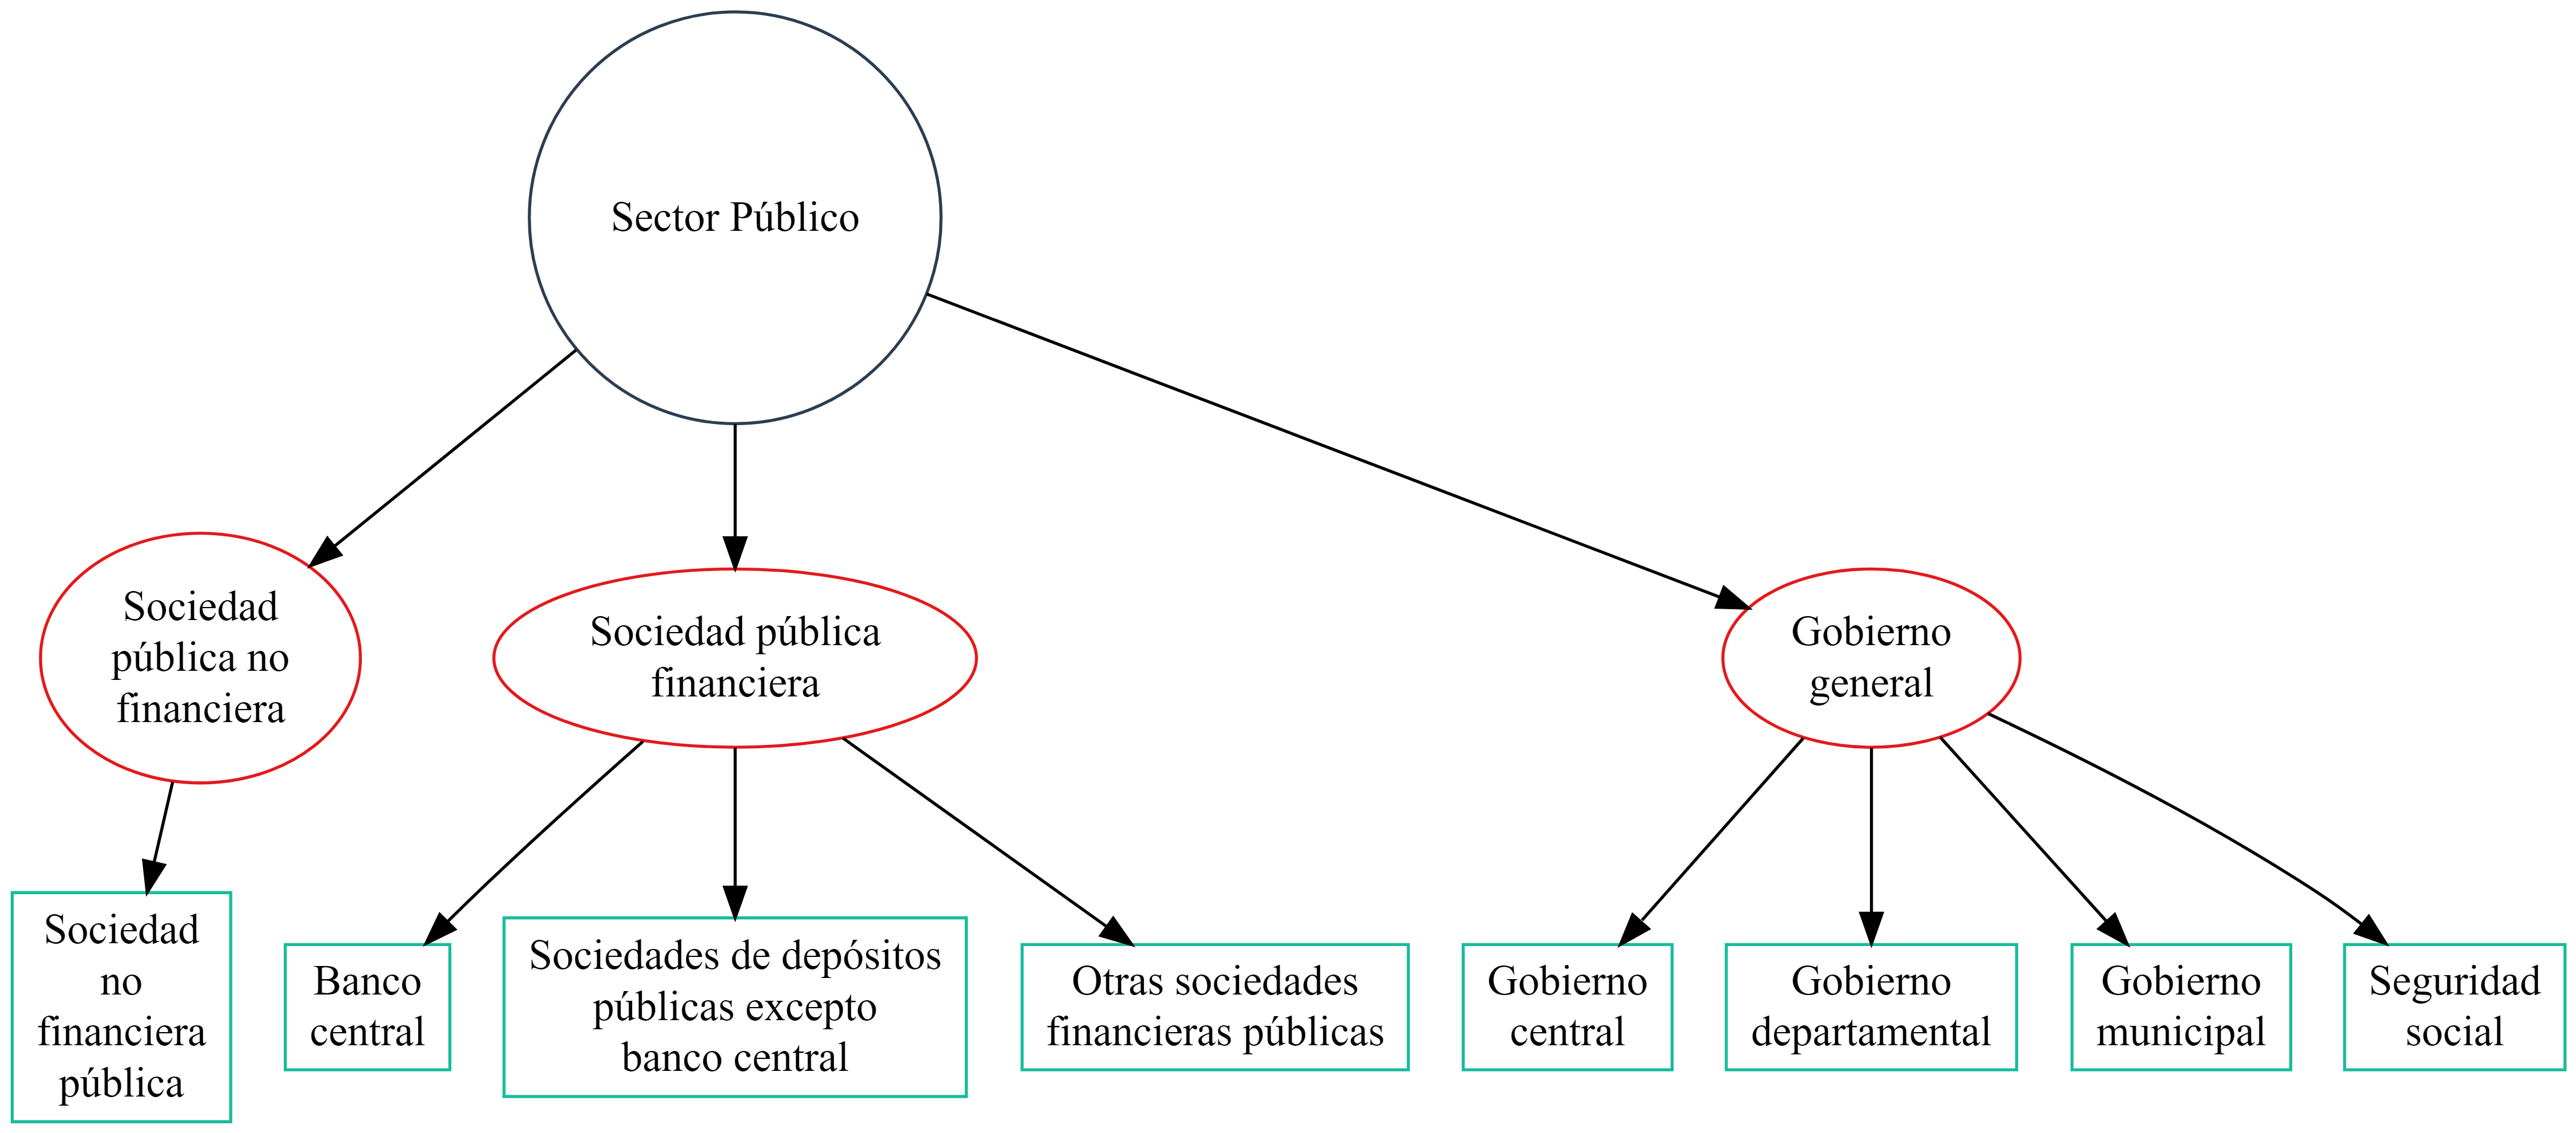
\includegraphics[width=5in,height=2in]{006_public_finances_files/figure-beamer/dot-figure-1.png}

}

\caption{\label{fig-division-public-sector-cuin-col}Division based on
(\citeproc{ref-international_monetary_fund_government_2014}{Fund 2014},
fig 2.3) and (\citeproc{ref-ciefp_clasificacion_2021}{CIEFP 2021}) using
the \textbf{Clasificación entidades según Código Único Institucional -
CUIN}}

\end{figure}%
\end{frame}

\begin{frame}{}
\phantomsection\label{section-5}
\begin{figure}

\centering{

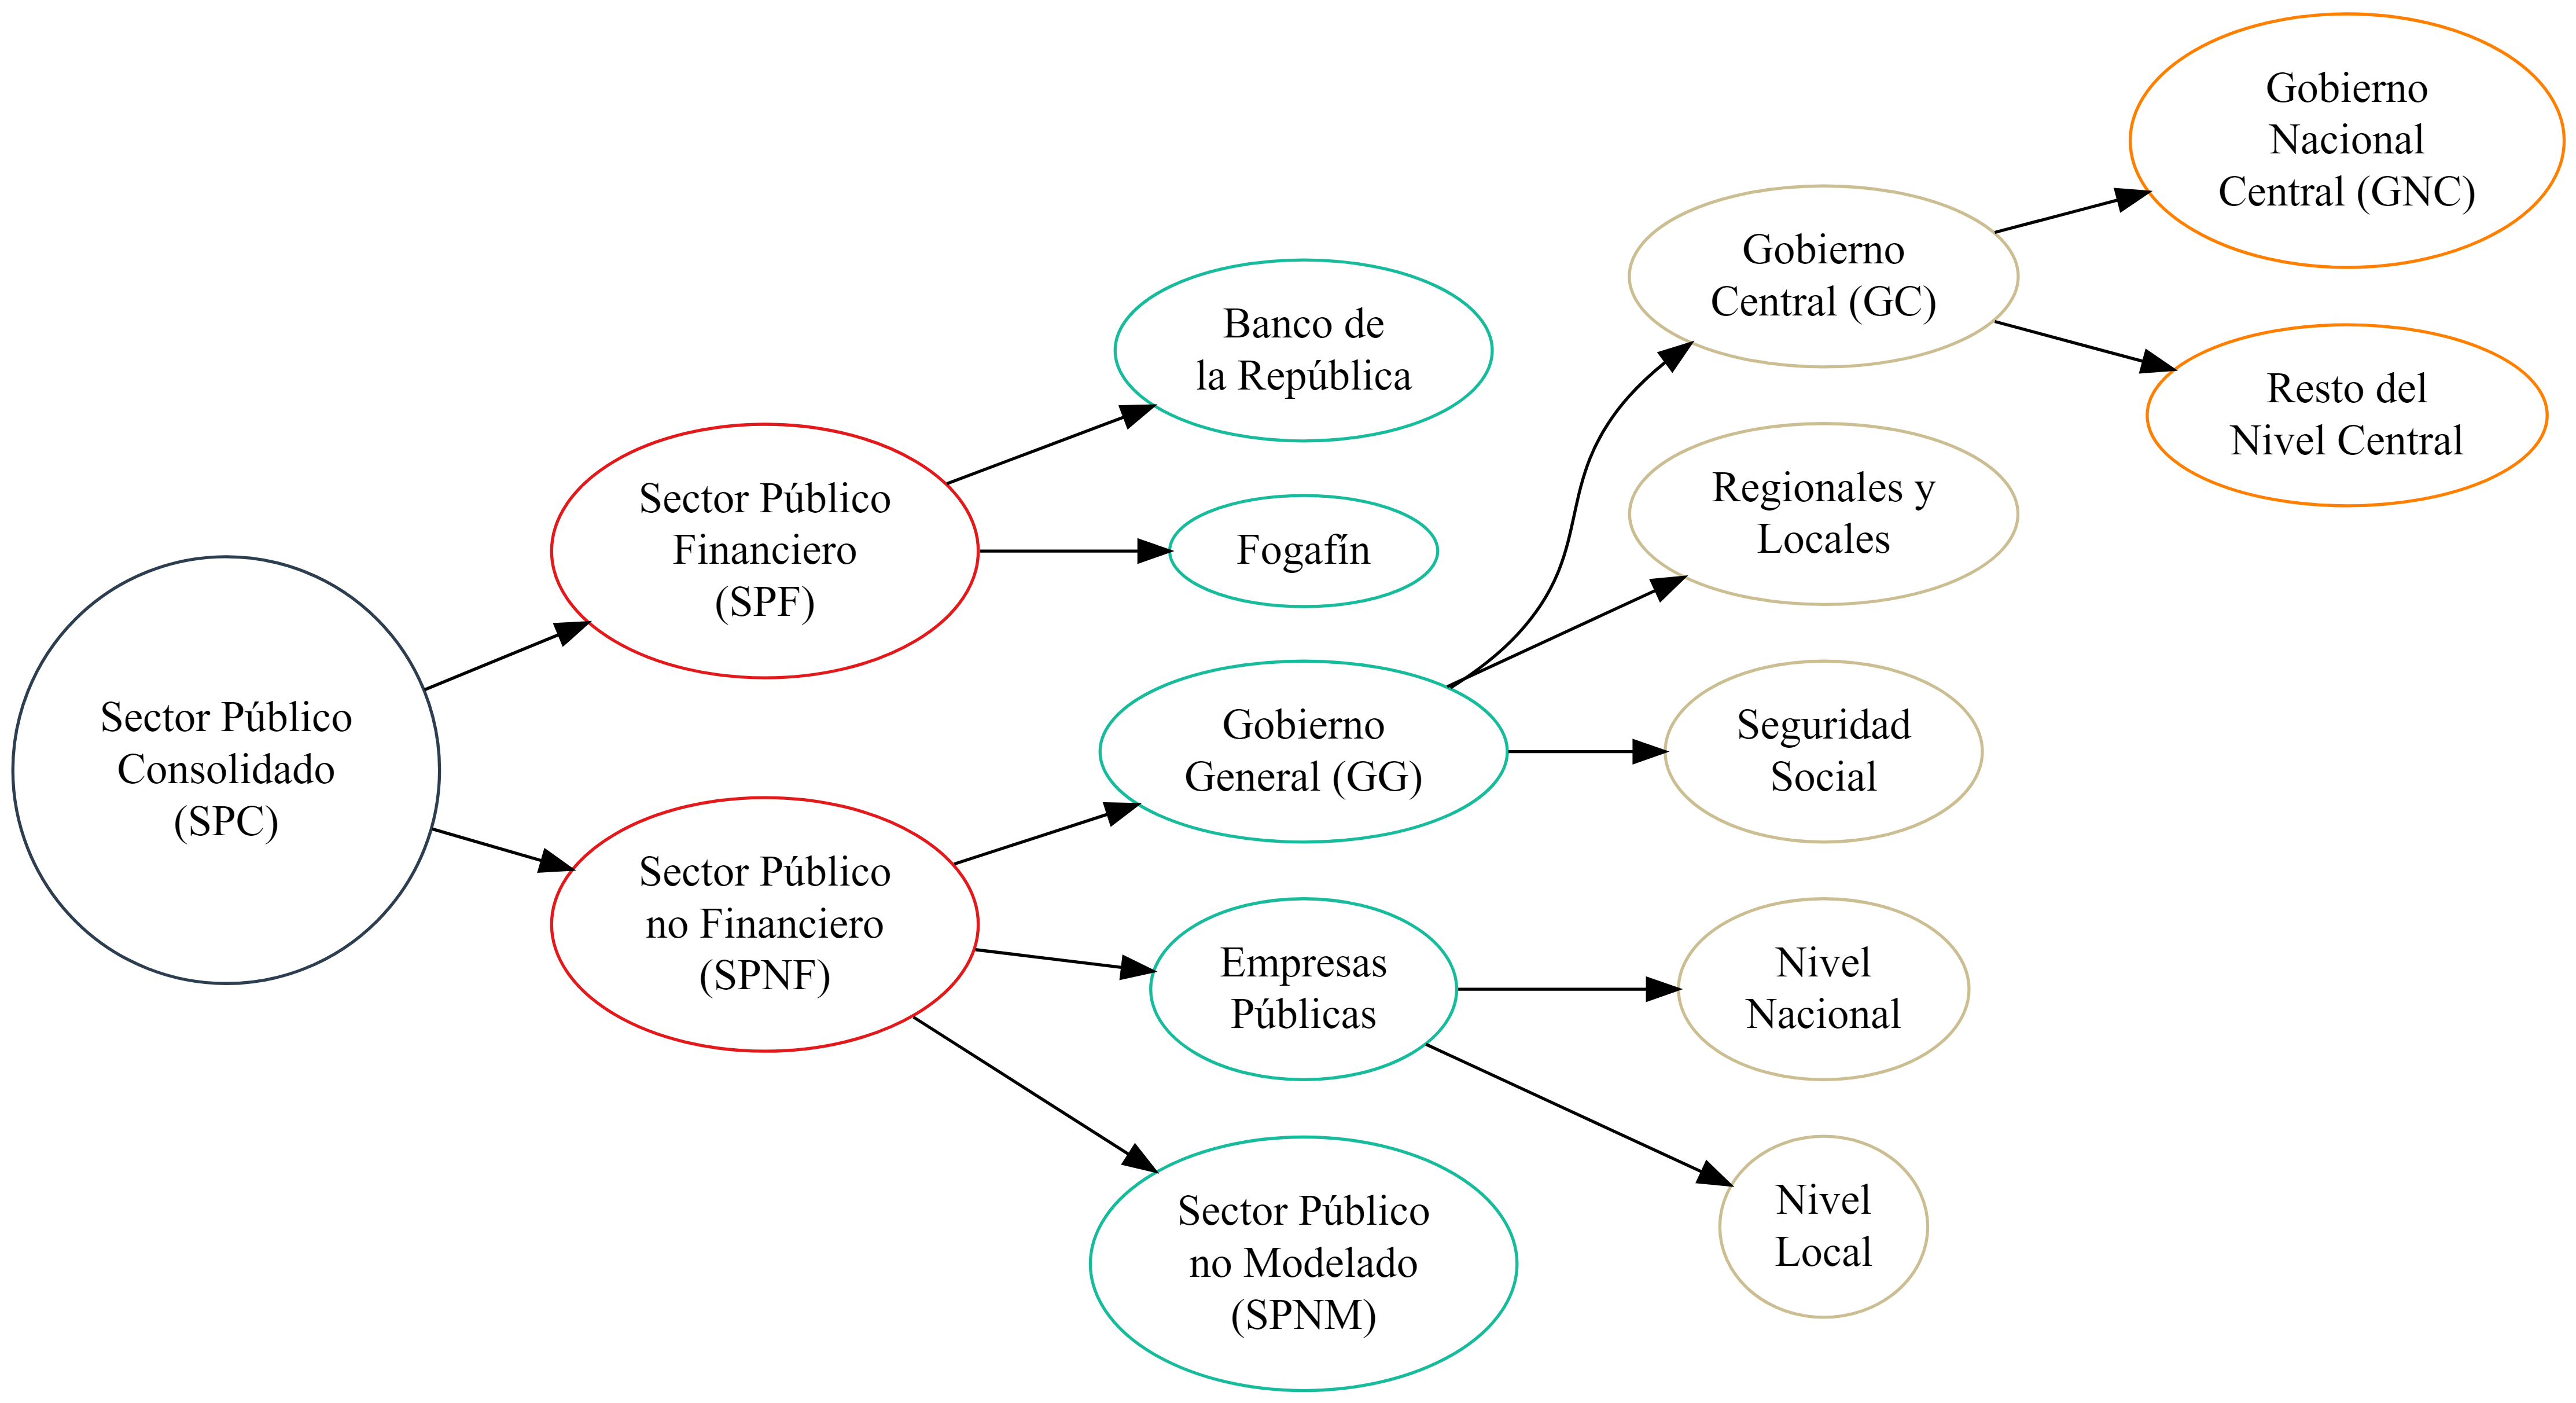
\includegraphics[width=5in,height=2in]{006_public_finances_files/figure-beamer/dot-figure-2.png}

}

\caption{\label{fig-division-public-sector-minhacienda-col}Division
based on how the difference balances are reported by
MinHacienda{[}\^{}1{]}}

\end{figure}%
\end{frame}

\begin{frame}{}
\phantomsection\label{section-6}
\begin{itemize}
\item
  Central National Government (Gobierno Nacional Central (GNC)) Fiscal
  Balance

  \begin{itemize}
  \item
    The fiscal balance is the difference between the central national
    government's revenues and its expenditures
  \item
    It shows the extent to which expenditure in a given year is financed
    by the revenues collected in that year
    (\citeproc{ref-oecd_government_2021}{OECD 2021}, p 68)

    \begin{itemize}
    \item
      When the central national government spends more than it collects
      as revenues, it has a \textbf{fiscal deficit}
    \item
      When the central national government spends less than it collects
      as revenues, it has a \textbf{fiscal surplus}
    \end{itemize}
  \end{itemize}
\end{itemize}
\end{frame}

\begin{frame}{}
\phantomsection\label{section-7}
\begin{table}

\caption{\label{tbl-ingresos-tributarios-no-tributarios-col}Ingresos
tributarios y no tributarios (\% PIB)}

\centering{

\centering\begingroup\fontsize{5.2}{7.2}\selectfont

\begin{threeparttable}
\begin{tabular}{lr}
\toprule
\textbf{Concepto} & \textbf{2023\textsuperscript{a}}\\
\midrule
\cellcolor[HTML]{CCBE93}{\textbf{INGRESOS CORRIENTES DE LA NACION}} & \cellcolor[HTML]{CCBE93}{\textbf{16.81}}\\
\cellcolor[HTML]{E31A1C}{\textbf{\hspace{2em}INGRESOS TRIBUTARIOS}} & \cellcolor[HTML]{E31A1C}{\textbf{16.74}}\\
\cellcolor[HTML]{18BC9C}{\textbf{\hspace{3em}DIAN}} & \cellcolor[HTML]{18BC9C}{\textbf{16.67}}\\
\hspace{5em}Renta & 8.87\\
\hspace{5em}IVA interno & 3.89\\
\hspace{5em}IVA externo & 2.11\\
\hspace{5em}Gravamen arancelario & 0.35\\
\hspace{5em}Sobretasa a la Importaciones CIF & 0.00\\
\hspace{5em}Imp. Nacional a la Gasolina y ACPM & 0.14\\
\hspace{5em}Impuesto al Carbono & 0.04\\
\hspace{5em}Consumo & 0.20\\
\hspace{5em}CREE & 0.01\\
\hspace{5em}Sobretasa a la Gasolina y ACPM & 0.00\\
\hspace{5em}Gravamen movimientos financieros & 0.87\\
\hspace{5em}Resto & 0.06\\
\hspace{5em}Timbre & 0.01\\
\hspace{5em}Impuesto SIMPLE & 0.10\\
\hspace{5em}Normalización & 0.00\\
\hspace{5em}Retención en la fuente inmuebles & 0.00\\
\hspace{5em}Contribución para la Democracia (Patrimonio) / Impuesto a la riqueza & 0.08\\
\cellcolor[HTML]{E31A1C}{\textbf{\hspace{2em}INGRESOS NO TRIBUTARIOS}} & \cellcolor[HTML]{E31A1C}{\textbf{0.08}}\\
\hspace{5em}Contribución de Hidrocarburos & 0.00\\
\hspace{5em}Concesiones & 0.00\\
\hspace{5em}Resto & 0.08\\
\bottomrule
\end{tabular}
\begin{tablenotes}
\item Source: Ministerio de Hacienda y Crédito Público - Balance Gobierno Nacional Central
\item Last update: 2024-05-28
\item[a] \%PIB - Cierre fiscal
\end{tablenotes}
\end{threeparttable}
\endgroup{}

}

\end{table}%
\end{frame}

\begin{frame}{}
\phantomsection\label{section-8}
\begin{table}

\caption{\label{tbl-ingresos-totales-col}Ingresos totales (\% PIB)}

\centering{

\centering\begingroup\fontsize{6}{8}\selectfont

\begin{threeparttable}
\begin{tabular}{lr}
\toprule
\textbf{Concepto} & \textbf{2023\textsuperscript{a}}\\
\midrule
\cellcolor[HTML]{CCBE93}{\textbf{1. INGRESOS TOTALES  (SIN CAUSADOS)}} & \cellcolor[HTML]{CCBE93}{\textbf{18.84}}\\
\textbf{\hspace{2em}INGRESOS CORRIENTES DE LA NACION} & \textbf{16.81}\\
\cellcolor[HTML]{18BC9C}{\hspace{3em}INGRESOS TRIBUTARIOS} & \cellcolor[HTML]{18BC9C}{16.74}\\
\hspace{3em}INGRESOS NO TRIBUTARIOS & 0.08\\
\textbf{\hspace{2em}FONDOS ESPECIALES} & \textbf{0.28}\\
\textbf{\hspace{2em}OTROS RECURSOS DE CAPITAL} & \textbf{1.75}\\
\hspace{5em}Rendimientos Financieros Totales & 0.02\\
\hspace{5em}Excedentes Financieros & 1.61\\
\hspace{7em}Ecopetrol & 1.37\\
\hspace{7em}Banco de la República & 0.10\\
\hspace{7em}Telecom & 0.00\\
\hspace{7em}Isa e Isagen & 0.00\\
\hspace{7em}Bancóldex & 0.00\\
\hspace{7em}Estapúblicos & 0.12\\
\hspace{7em}Resto de empresas & 0.03\\
\hspace{5em}Recuperación de cartera diferente SPNF & 0.03\\
\hspace{5em}Otros recursos & 0.09\\
\hspace{7em}Reintegros y recursos no apropiados & 0.15\\
\hspace{7em}Resto & -0.07\\
\bottomrule
\end{tabular}
\begin{tablenotes}
\item Source: Ministerio de Hacienda y Crédito Público - Balance Gobierno Nacional Central
\item Last update: 2024-05-28
\item[a] \%PIB - Cierre fiscal
\end{tablenotes}
\end{threeparttable}
\endgroup{}

}

\end{table}%
\end{frame}

\begin{frame}{}
\phantomsection\label{section-9}
\begin{table}

\caption{\label{tbl-ingresos-pagos-totales-col}Ingresos y pagos totales
(\% PIB)}

\centering{

\centering\begingroup\fontsize{5.5}{7.5}\selectfont

\begin{threeparttable}
\begin{tabular}{lr}
\toprule
\textbf{Concepto} & \textbf{2023\textsuperscript{a}}\\
\midrule
\cellcolor[HTML]{CCBE93}{\textbf{1. INGRESOS TOTALES  (SIN CAUSADOS)}} & \cellcolor[HTML]{CCBE93}{\textbf{18.84}}\\
\hspace{2em}INGRESOS CORRIENTES DE LA NACION & 16.81\\
\cellcolor[HTML]{18BC9C}{\hspace{3em}INGRESOS TRIBUTARIOS} & \cellcolor[HTML]{18BC9C}{16.74}\\
\hspace{3em}INGRESOS NO TRIBUTARIOS & 0.08\\
\hspace{2em}FONDOS ESPECIALES & 0.28\\
\hspace{2em}OTROS RECURSOS DE CAPITAL & 1.75\\
\cellcolor[HTML]{CCBE93}{\textbf{2. PAGOS TOTALES}} & \cellcolor[HTML]{CCBE93}{\textbf{22.11}}\\
\cellcolor[HTML]{E31A1C}{\textbf{\hspace{2em}PAGOS TOTALES SIN INTERESES}} & \cellcolor[HTML]{E31A1C}{\textbf{16.57}}\\
\cellcolor[HTML]{E31A1C}{\textbf{\hspace{2em}PAGOS CORRIENTES DE LA NACION}} & \cellcolor[HTML]{E31A1C}{\textbf{19.49}}\\
\hspace{3em}INTERESES & 2.92\\
\hspace{5em}Intereses deuda externa & 0.88\\
\hspace{5em}Intereses deuda interna & 2.04\\
\hspace{5em}Costo impuesto endeudamiento externo & 0.00\\
\hspace{3em}FUNCIONAMIENTO & 16.57\\
\hspace{4em}Servicios personales & 2.09\\
\cellcolor[HTML]{18BC9C}{\hspace{4em}Transferencias} & \cellcolor[HTML]{18BC9C}{13.81}\\
\hspace{5em}Transferencias regionales (SGP desde 2002) & 3.36\\
\hspace{5em}Pensiones & 3.37\\
\hspace{5em}Otras & 7.08\\
\hspace{4em}Gastos generales y otros & 0.68\\
\cellcolor[HTML]{E31A1C}{\textbf{\hspace{2em}INVERSION}} & \cellcolor[HTML]{E31A1C}{\textbf{2.62}}\\
\bottomrule
\end{tabular}
\begin{tablenotes}
\item Source: Ministerio de Hacienda y Crédito Público - Balance Gobierno Nacional Central
\item Last update: 2024-05-28
\item[a] \%PIB - Cierre fiscal
\end{tablenotes}
\end{threeparttable}
\endgroup{}

}

\end{table}%
\end{frame}

\begin{frame}{}
\phantomsection\label{section-10}
\begin{table}

\caption{\label{tbl-balance-fiscal-gobierno-nacional-central-pct-pib-col}Balance
fiscal gobierno nacional central (\% PIB)}

\centering{

\centering\begingroup\fontsize{5.5}{7.5}\selectfont

\begin{threeparttable}
\begin{tabular}{lr}
\toprule
\textbf{Concepto} & \textbf{2023\textsuperscript{a}}\\
\midrule
\cellcolor[HTML]{CCBE93}{\textbf{1. INGRESOS TOTALES  (SIN CAUSADOS)}} & \cellcolor[HTML]{CCBE93}{\textbf{18.84}}\\
\hspace{2em}INGRESOS CORRIENTES DE LA NACION & 16.81\\
\hspace{3em}INGRESOS TRIBUTARIOS & 16.74\\
\hspace{3em}INGRESOS NO TRIBUTARIOS & 0.08\\
\hspace{2em}FONDOS ESPECIALES & 0.28\\
\hspace{2em}OTROS RECURSOS DE CAPITAL & 1.75\\
\cellcolor[HTML]{CCBE93}{\textbf{2. PAGOS TOTALES}} & \cellcolor[HTML]{CCBE93}{\textbf{22.11}}\\
\hspace{2em}PAGOS TOTALES SIN INTERESES & 16.57\\
\hspace{2em}PAGOS CORRIENTES DE LA NACION & 19.49\\
\cellcolor[HTML]{18BC9C}{\textbf{\hspace{3em}INTERESES}} & \cellcolor[HTML]{18BC9C}{\textbf{2.92}}\\
\hspace{3em}FUNCIONAMIENTO & 16.57\\
\hspace{2em}INVERSION & 2.62\\
\cellcolor[HTML]{CCBE93}{\textbf{3. DEFICIT O SUPERAVIT EFECTIVO}} & \cellcolor[HTML]{CCBE93}{\textbf{-3.27}}\\
\hspace{2em}PRESTAMO NETO & 0.00\\
\hspace{2em}INGRESOS CAUSADOS & 0.00\\
\cellcolor[HTML]{18BC9C}{\textbf{\hspace{2em}GASTOS CAUSADOS}} & \cellcolor[HTML]{18BC9C}{\textbf{0.99}}\\
\hspace{2em}DEUDA FLOTANTE & 0.00\\
\cellcolor[HTML]{CCBE93}{\textbf{4. DEFICIT O SUPERAVIT TOTAL}} & \cellcolor[HTML]{CCBE93}{\textbf{-4.26}}\\
\cellcolor[HTML]{CCBE93}{\textbf{5. COSTOS DE LA REEST. FINANCIERA}} & \cellcolor[HTML]{CCBE93}{\textbf{0.00}}\\
\cellcolor[HTML]{E31A1C}{\textbf{6. DEFICIT A FINANCIAR}} & \cellcolor[HTML]{E31A1C}{\textbf{-4.26}}\\
\cellcolor[HTML]{CAB2D6}{\textbf{BALANCE PRIMARIO}} & \cellcolor[HTML]{CAB2D6}{\textbf{-0.35}}\\
\bottomrule
\end{tabular}
\begin{tablenotes}
\item Source: Ministerio de Hacienda y Crédito Público - Balance Gobierno Nacional Central
\item Last update: 2024-05-28
\item[a] \%PIB - Cierre fiscal
\end{tablenotes}
\end{threeparttable}
\endgroup{}

}

\end{table}%
\end{frame}

\begin{frame}{}
\phantomsection\label{section-11}
\begin{table}

\caption{\label{tbl-balance-fiscal-gobierno-nacional-central-col}Balance
fiscal gobierno nacional central (COP)}

\centering{

\centering\begingroup\fontsize{5.5}{7.5}\selectfont

\begin{threeparttable}
\begin{tabular}{ll}
\toprule
\textbf{Concepto} & \textbf{2023\textsuperscript{a}}\\
\midrule
\cellcolor[HTML]{CCBE93}{\textbf{1. INGRESOS TOTALES  (SIN CAUSADOS)}} & \cellcolor[HTML]{CCBE93}{\textbf{296,365,315,838,095.9}}\\
\hspace{2em}INGRESOS CORRIENTES DE LA NACION & 264,387,228,958,374.0\\
\hspace{3em}INGRESOS TRIBUTARIOS & 263,189,938,236,485.4\\
\hspace{3em}INGRESOS NO TRIBUTARIOS & 1,197,290,721,888.6\\
\hspace{2em}FONDOS ESPECIALES & 4,404,531,097,792.0\\
\hspace{2em}OTROS RECURSOS DE CAPITAL & 27,573,555,781,929.9\\
\cellcolor[HTML]{CCBE93}{\textbf{2. PAGOS TOTALES}} & \cellcolor[HTML]{CCBE93}{\textbf{347,761,455,208,728.3}}\\
\hspace{2em}PAGOS TOTALES SIN INTERESES & 260,641,563,447,192.5\\
\hspace{2em}PAGOS CORRIENTES DE LA NACION & 306,543,938,313,804.6\\
\cellcolor[HTML]{18BC9C}{\textbf{\hspace{3em}INTERESES}} & \cellcolor[HTML]{18BC9C}{\textbf{45,902,374,866,612.1}}\\
\hspace{3em}FUNCIONAMIENTO & 260,641,563,447,192.4\\
\hspace{2em}INVERSION & 41,217,516,894,923.8\\
\cellcolor[HTML]{CCBE93}{\textbf{3. DEFICIT O SUPERAVIT EFECTIVO}} & \cellcolor[HTML]{CCBE93}{\textbf{-51,396,139,370,632.4}}\\
\hspace{2em}PRESTAMO NETO & -64,923,618,060.3\\
\hspace{2em}INGRESOS CAUSADOS & 0.0\\
\cellcolor[HTML]{18BC9C}{\textbf{\hspace{2em}GASTOS CAUSADOS}} & \cellcolor[HTML]{18BC9C}{\textbf{15,565,729,479,504.4}}\\
\hspace{2em}DEUDA FLOTANTE & 19,706,817,372.5\\
\cellcolor[HTML]{CCBE93}{\textbf{4. DEFICIT O SUPERAVIT TOTAL}} & \cellcolor[HTML]{CCBE93}{\textbf{-66,916,652,049,449.0}}\\
\cellcolor[HTML]{CCBE93}{\textbf{5. COSTOS DE LA REEST. FINANCIERA}} & \cellcolor[HTML]{CCBE93}{\textbf{0.0}}\\
\cellcolor[HTML]{E31A1C}{\textbf{6. DEFICIT A FINANCIAR}} & \cellcolor[HTML]{E31A1C}{\textbf{-66,916,652,049,449.0}}\\
\cellcolor[HTML]{CAB2D6}{\textbf{BALANCE PRIMARIO}} & \cellcolor[HTML]{CAB2D6}{\textbf{-5,448,547,703,332.5}}\\
\bottomrule
\end{tabular}
\begin{tablenotes}
\item Source: Ministerio de Hacienda y Crédito Público - Balance Gobierno Nacional Central
\item Last update: 2024-05-28
\item[a] Pesos colombianos (COP)
\end{tablenotes}
\end{threeparttable}
\endgroup{}

}

\end{table}%
\end{frame}

\section{Revenues: taxes}\label{revenues-taxes}

\begin{frame}{}
\phantomsection\label{section-12}
\begin{itemize}
\item
  Useful resources

  \begin{itemize}
  \item
    \textbf{Global Revenue Statistics Database}

    \begin{itemize}
    \tightlist
    \item
      \href{https://data-explorer.oecd.org/}{\textbf{https://data-explorer.oecd.org/}}
      \textgreater{} Taxation \textgreater{} Global tax revenues
      \textgreater{} Comparative tables of Revenue Statistics in Latin
      America and the Caribbean
    \end{itemize}
  \item
    \textbf{Guía ciudadana a la tributación y el gasto del Estado
    colombiano}
    (\citeproc{ref-observatorio_fiscal_de_la_universidad_javeriana_guiciudadana_2018}{Universidad
    Javeriana 2018})

    \begin{itemize}
    \tightlist
    \item
      \href{https://www.ofiscal.org/publicaciones}{\textbf{https://www.ofiscal.org/publicaciones}}
      \textgreater{} guías ciudadanas \textgreater{} Tributación y gasto
      del Estado colombiano \textgreater{} ver y descargar ↓
    \end{itemize}
  \end{itemize}
\end{itemize}
\end{frame}

\begin{frame}{}
\phantomsection\label{section-13}
\begin{itemize}
\item
  \textbf{Taxes}: ``compulsory unrequited payments to the general
  government or to a supranational authority''
  (\citeproc{ref-oecd_revenue_2020}{OECD 2020, 319})

  \begin{itemize}
  \item
    \emph{``Taxes are unrequited in the sense that benefits provided by
    government to taxpayers are not normally in proportion to their
    payments''} (\citeproc{ref-oecd_revenue_2020}{OECD 2020}, p 319)
  \item
    \emph{``The term \textbf{tax} does not include fines, penalties and
    compulsory loans paid to government''}
    (\citeproc{ref-oecd_revenue_2020}{OECD 2020}, p 319)
  \item
    Compulsory social security contributions and paid to general
    government are treated here as tax revenues
    (\citeproc{ref-oecd_revenue_2020}{OECD 2020}, p 320)
  \end{itemize}
\end{itemize}
\end{frame}

\begin{frame}{}
\phantomsection\label{section-14}
\begin{itemize}
\item
  \textbf{Classification of Taxes by the OECD}
  (\citeproc{ref-oecd_revenue_2020}{OECD 2020, 317--18})

  \begin{itemize}
  \tightlist
  \item
    1000 Taxes on income, profits and capital gains (Impuestos sobre la
    renta, las utilidades y las ganancias de capital)
  \item
    2000 Social security contributions (Contribuciones a la seguridad
    social)
  \item
    3000 Taxes on payroll and workforce (Impuestos sobre la nómina y la
    fuerza de trabajo)
  \item
    4000 Taxes on property (Impuestos sobre la propiedad)
  \item
    5000 Taxes on goods and services (Impuestos sobre los bienes y
    servicios)
  \item
    6000 Other taxes (Otros impuestos)
  \end{itemize}
\end{itemize}
\end{frame}

\begin{frame}{}
\phantomsection\label{section-15}
\begin{itemize}
\item
  According to the Colombia's political constitution:

  \begin{itemize}
  \tightlist
  \item
    \emph{``ARTICULO 363. El sistema tributario se funda en los
    principios de \textbf{equidad}, \textbf{eficiencia} y
    \textbf{progresividad}. \ldots{}''}
  \end{itemize}
\item
  \textbf{Equity}
\end{itemize}

\begin{figure}

\begin{minipage}{0.50\linewidth}

\centering{

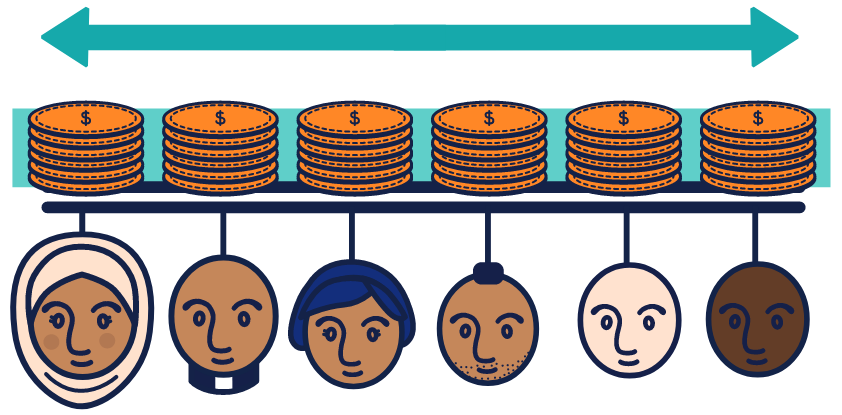
\includegraphics[width=1.875in,height=1.875in]{_000_images/006_horizontal_equity.png}

}

\subcaption{\label{fig-horizontal}Horizontal}

\end{minipage}%
%
\begin{minipage}{0.50\linewidth}

\centering{

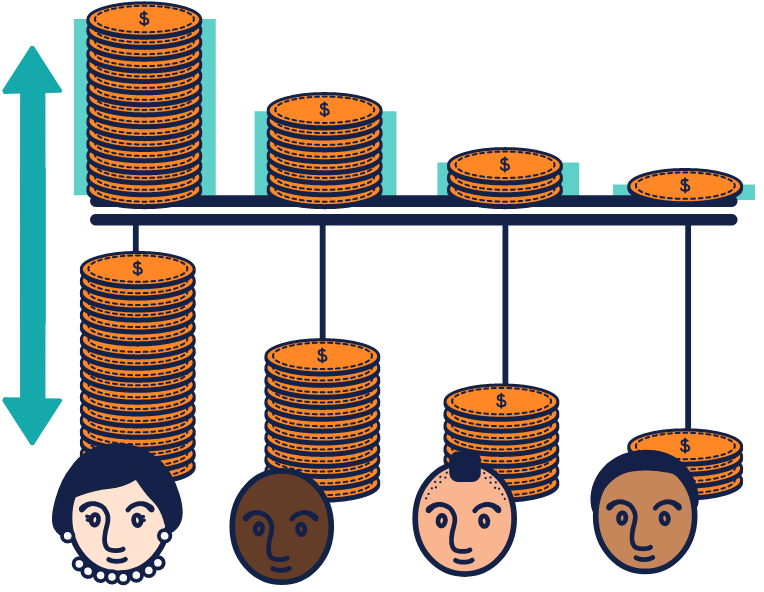
\includegraphics[width=1.875in,height=1.875in]{_000_images/006_vertical_equity.png}

}

\subcaption{\label{fig-vertical}Vertical}

\end{minipage}%

\caption{\label{fig-horizontal_vs_vertical_equity}Horizontal and
vertical
(\citeproc{ref-observatorio_fiscal_de_la_universidad_javeriana_guiciudadana_2018}{Universidad
Javeriana 2018, 8})}

\end{figure}%
\end{frame}

\begin{frame}{}
\phantomsection\label{section-16}
\begin{itemize}
\tightlist
\item
  \textbf{Efficiency}: taxes change the behavior of individuals and
  sometimes distort the economic activity by creating a deadweight loss.
  Therefore the idea is to have a tax system that minimize or mitigate
  these negative effects
\end{itemize}
\end{frame}

\begin{frame}{}
\phantomsection\label{section-17}
\begin{itemize}
\tightlist
\item
  \textbf{Progressivity}
\end{itemize}

\footnotesize

\begin{figure}

\begin{minipage}{0.45\linewidth}

\centering{

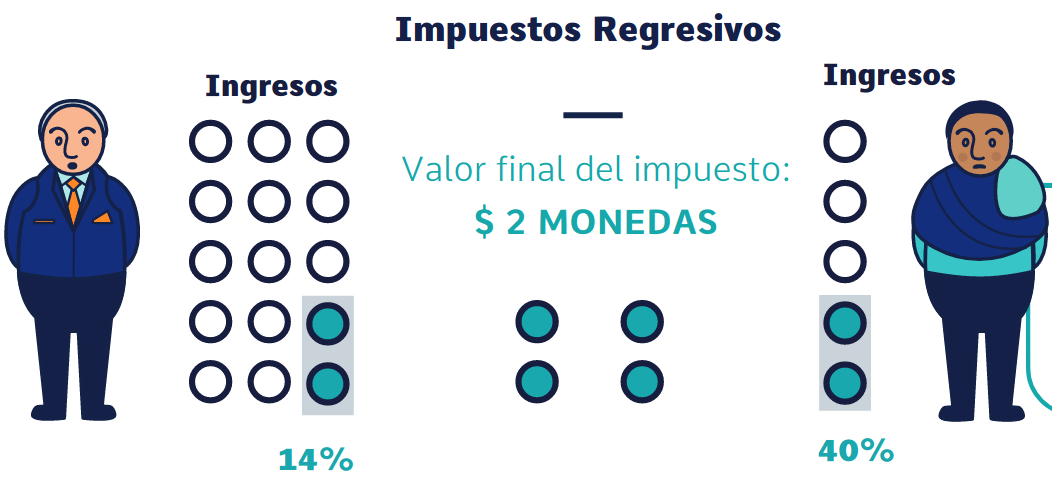
\includegraphics[width=1.5625in,height=1.5625in]{_000_images/006_regressive_tax.png}

}

\subcaption{\label{fig-regressive}Regressive}

\end{minipage}%
%
\begin{minipage}{0.10\linewidth}
~\end{minipage}%
%
\begin{minipage}{0.45\linewidth}

\centering{

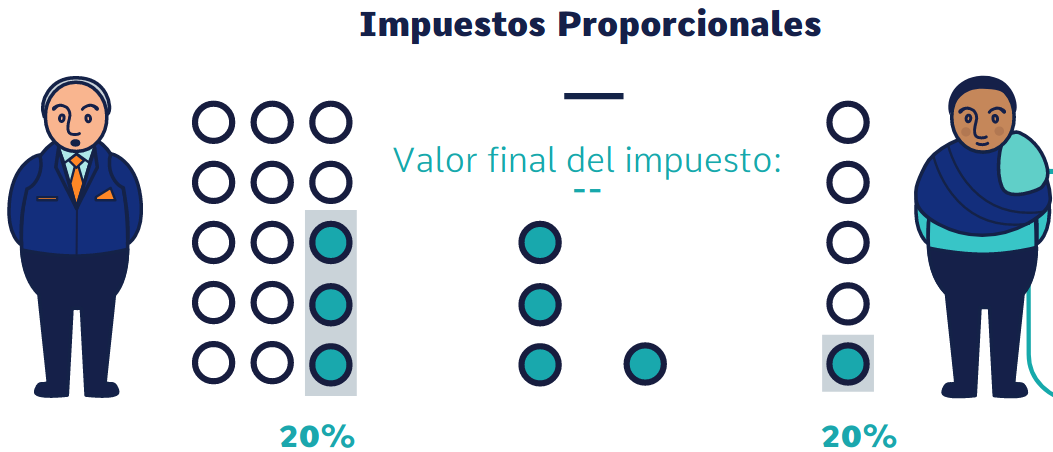
\includegraphics[width=1.5625in,height=1.5625in]{_000_images/006_proportional_tax.png}

}

\subcaption{\label{fig-proportional}Proportional}

\end{minipage}%
\newline
\begin{minipage}{0.30\linewidth}
~\end{minipage}%
%
\begin{minipage}{0.40\linewidth}

\centering{

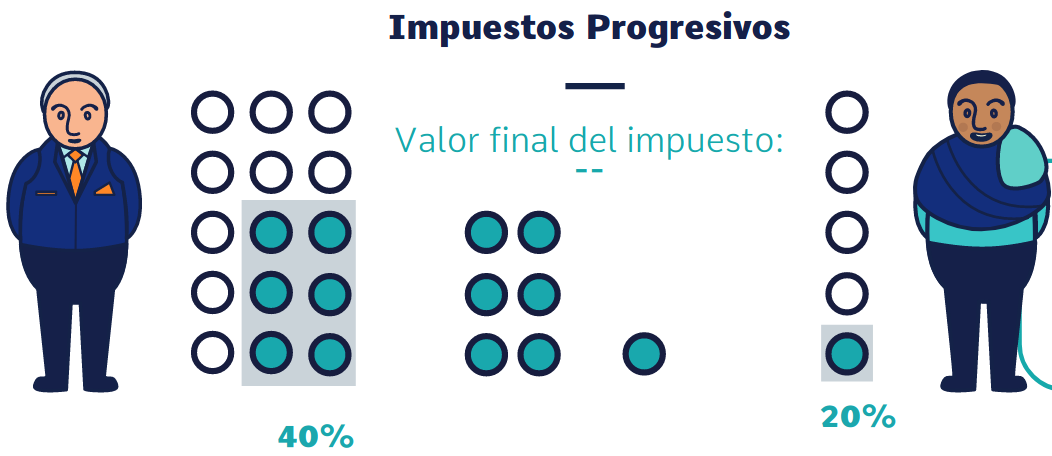
\includegraphics[width=1.5625in,height=1.5625in]{_000_images/006_progressive_tax.png}

}

\subcaption{\label{fig-progressive}Progressive}

\end{minipage}%
%
\begin{minipage}{0.30\linewidth}
~\end{minipage}%

\caption{\label{fig-regressive_proportional_progressive}Regressive,
proportional and progressive tax
(\citeproc{ref-observatorio_fiscal_de_la_universidad_javeriana_guiciudadana_2018}{Universidad
Javeriana 2018, 11})}

\end{figure}%
\end{frame}

\begin{frame}{}
\phantomsection\label{section-18}
\begin{figure}

\centering{

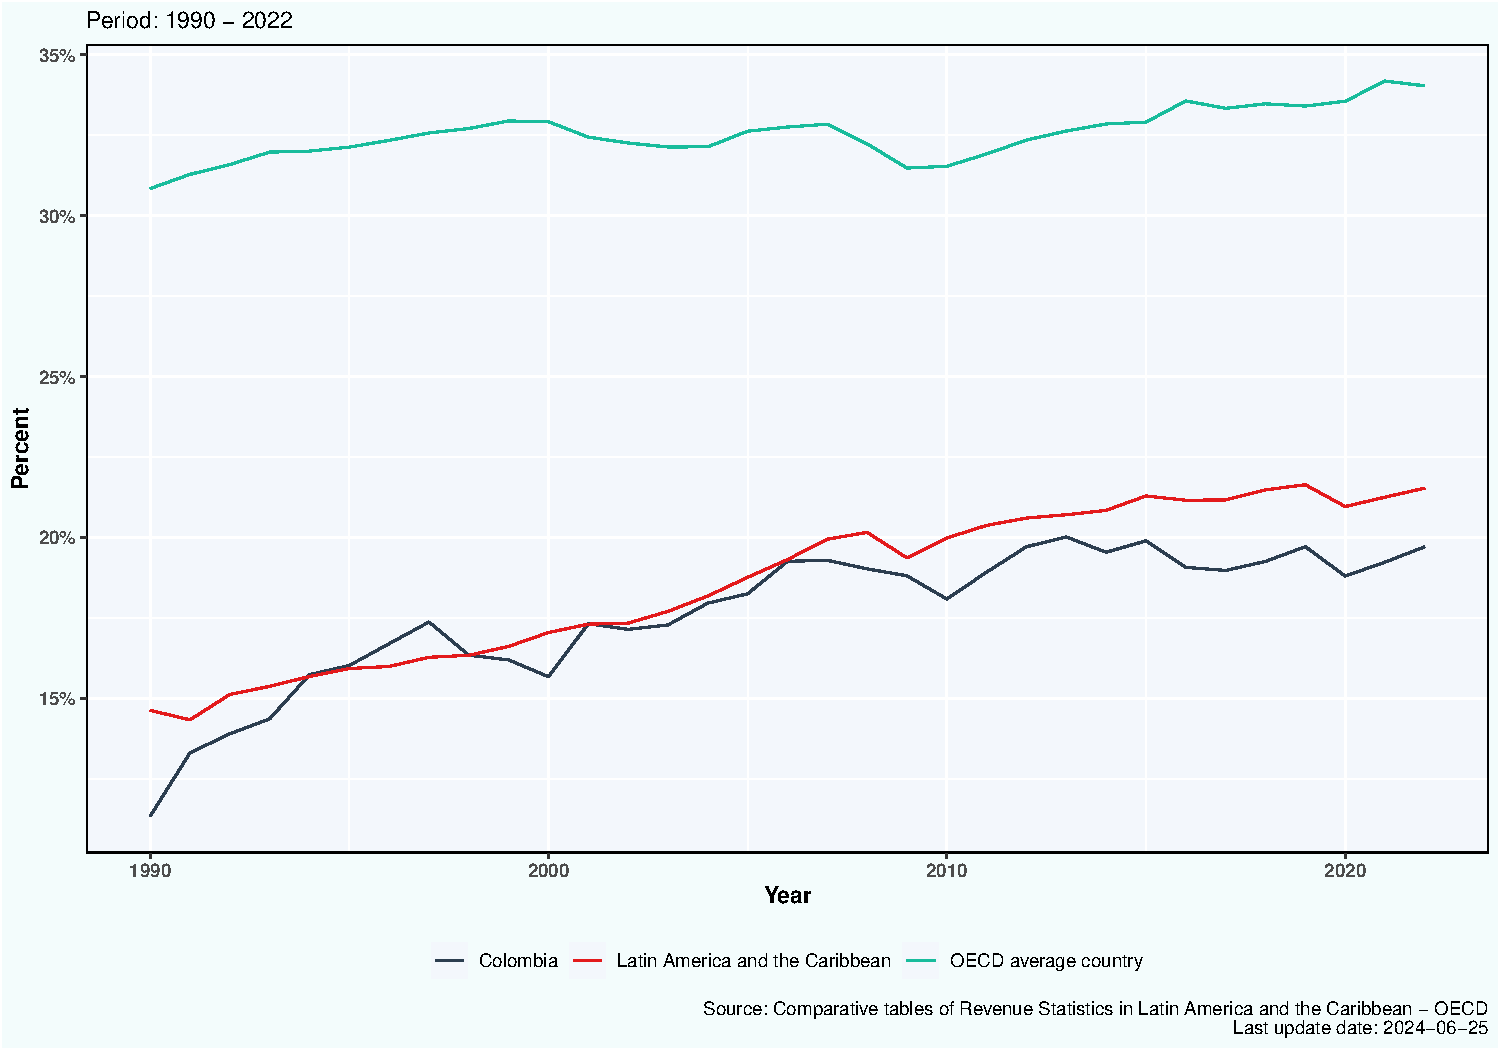
\includegraphics[width=0.85\textwidth,height=\textheight]{006_public_finances_files/figure-beamer/fig-total-tax-revenue-pct-gdp-col-lac-oecd-1.pdf}

}

\caption{\label{fig-total-tax-revenue-pct-gdp-col-lac-oecd}Total tax
revenue as \% of Gross Domestic Product}

\end{figure}%
\end{frame}

\begin{frame}{}
\phantomsection\label{section-19}
\begin{figure}

\centering{

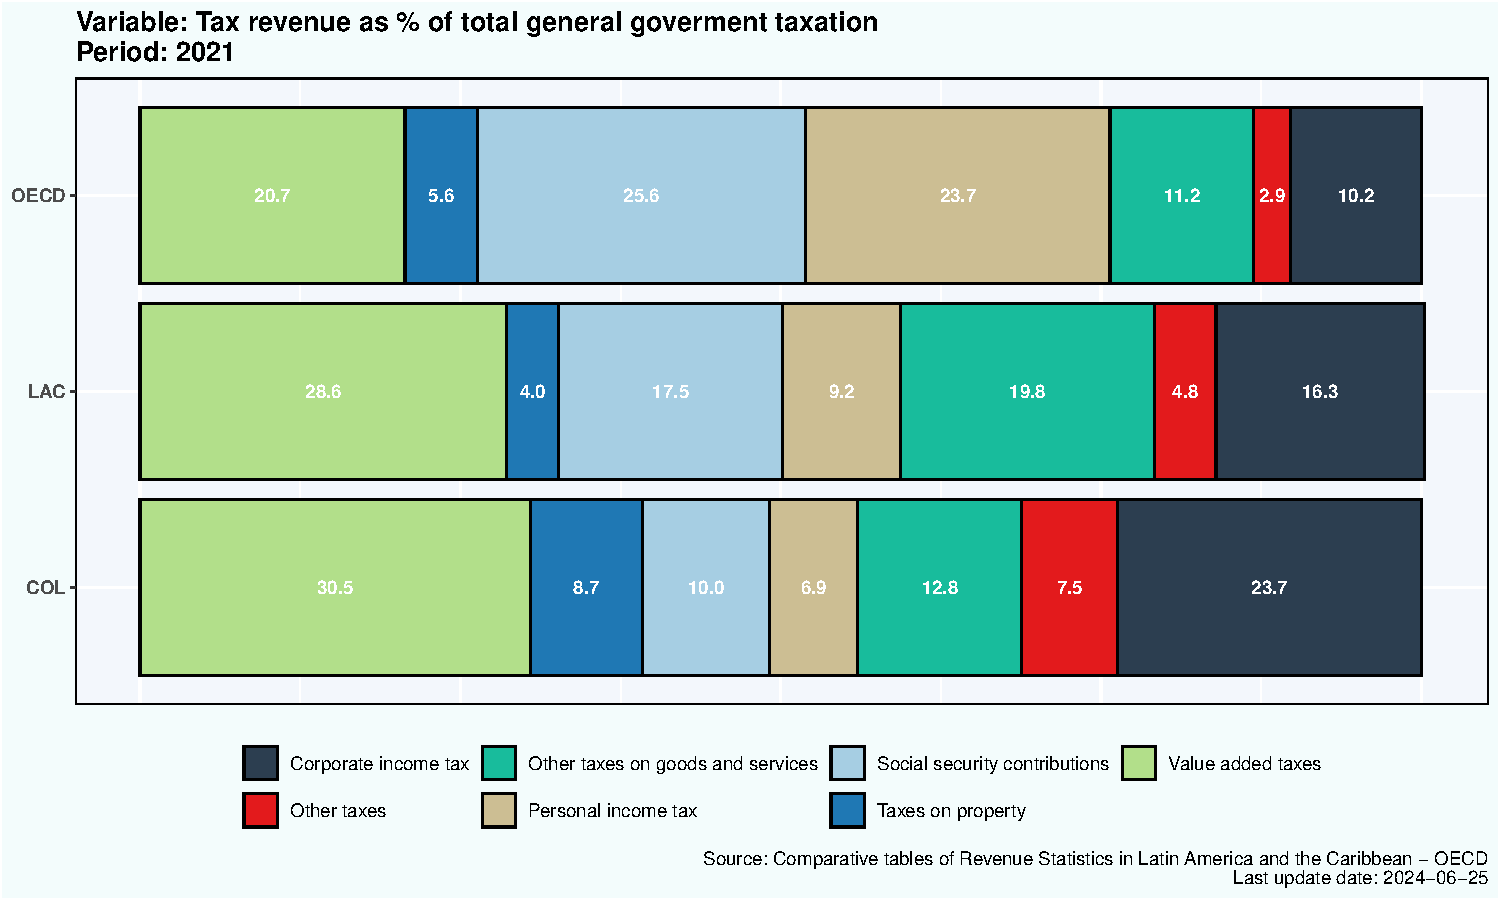
\includegraphics[width=0.85\textwidth,height=\textheight]{006_public_finances_files/figure-beamer/fig-tax-structure-col-lac-oecd-1.pdf}

}

\caption{\label{fig-tax-structure-col-lac-oecd}Tax structures for
Colombia (COL), Latin America and the Caribbean (LAC) and OECD}

\end{figure}%
\end{frame}

\section{Expenditures}\label{expenditures}

\begin{frame}{}
\phantomsection\label{section-20}
\begin{itemize}
\item
  Useful resources

  \begin{itemize}
  \item
    \textbf{Portal de transparencia económica}

    \begin{itemize}
    \tightlist
    \item
      \href{https://www.pte.gov.co}{\textbf{https://www.pte.gov.co}}
      \textgreater{} PRESUPUESTO GENERAL DE LA NACIÓN \textgreater{}
      Ejecución
    \end{itemize}
  \item
    \textbf{Guía ciudadana a la tributación y el gasto del Estado
    colombiano}
    (\citeproc{ref-observatorio_fiscal_de_la_universidad_javeriana_guiciudadana_2018}{Universidad
    Javeriana 2018})

    \begin{itemize}
    \tightlist
    \item
      \href{https://www.ofiscal.org/publicaciones}{\textbf{https://www.ofiscal.org/publicaciones}}
      \textgreater{} guías ciudadanas \textgreater{} Tributación y gasto
      del Estado colombiano \textgreater{} ver y descargar ↓
    \end{itemize}
  \item
    \textbf{Presupuesto en Perspectiva Económica (PePE)}

    \begin{itemize}
    \tightlist
    \item
      \href{https://www.ofiscal.org/}{\textbf{https://www.ofiscal.org/}}
      \textgreater{} Interactúa \textgreater{} PePE
    \end{itemize}
  \end{itemize}
\end{itemize}
\end{frame}

\begin{frame}{}
\phantomsection\label{section-21}
\begin{itemize}
\item
  \textbf{Presupuesto General de la Nación (PGN)}

  \begin{itemize}
  \item
    It is the most important financial management instrument of fiscal
    policy
  \item
    This instrument presents the government's proposed revenues and
    spending for a specific period
  \item
    Every year the ``Presupuesto General de la Nación (PGN)'' is define
    for the next year
  \item
    The ``Presupuesto General de la Nación (PGN)'' must be approved by
    the congress and sanctioned as a law by the president
  \item
    For more information check out \textbf{Guía ciudadana al Presupuesto
    General de la Nación}
    (\citeproc{ref-observatorio_fiscal_de_la_universidad_javeriana_guiciudadana_2022}{Universidad
    Javeriana 2022})

    \begin{itemize}
    \tightlist
    \item
      \href{https://www.ofiscal.org/}{\textbf{https://www.ofiscal.org/}}
      \textgreater{} Guias \textgreater{} Presupuesto General de la
      Nación \textgreater{} ver y descargar ↓
    \end{itemize}
  \end{itemize}
\end{itemize}
\end{frame}

\begin{frame}{}
\phantomsection\label{section-22}
\begin{figure}

\centering{

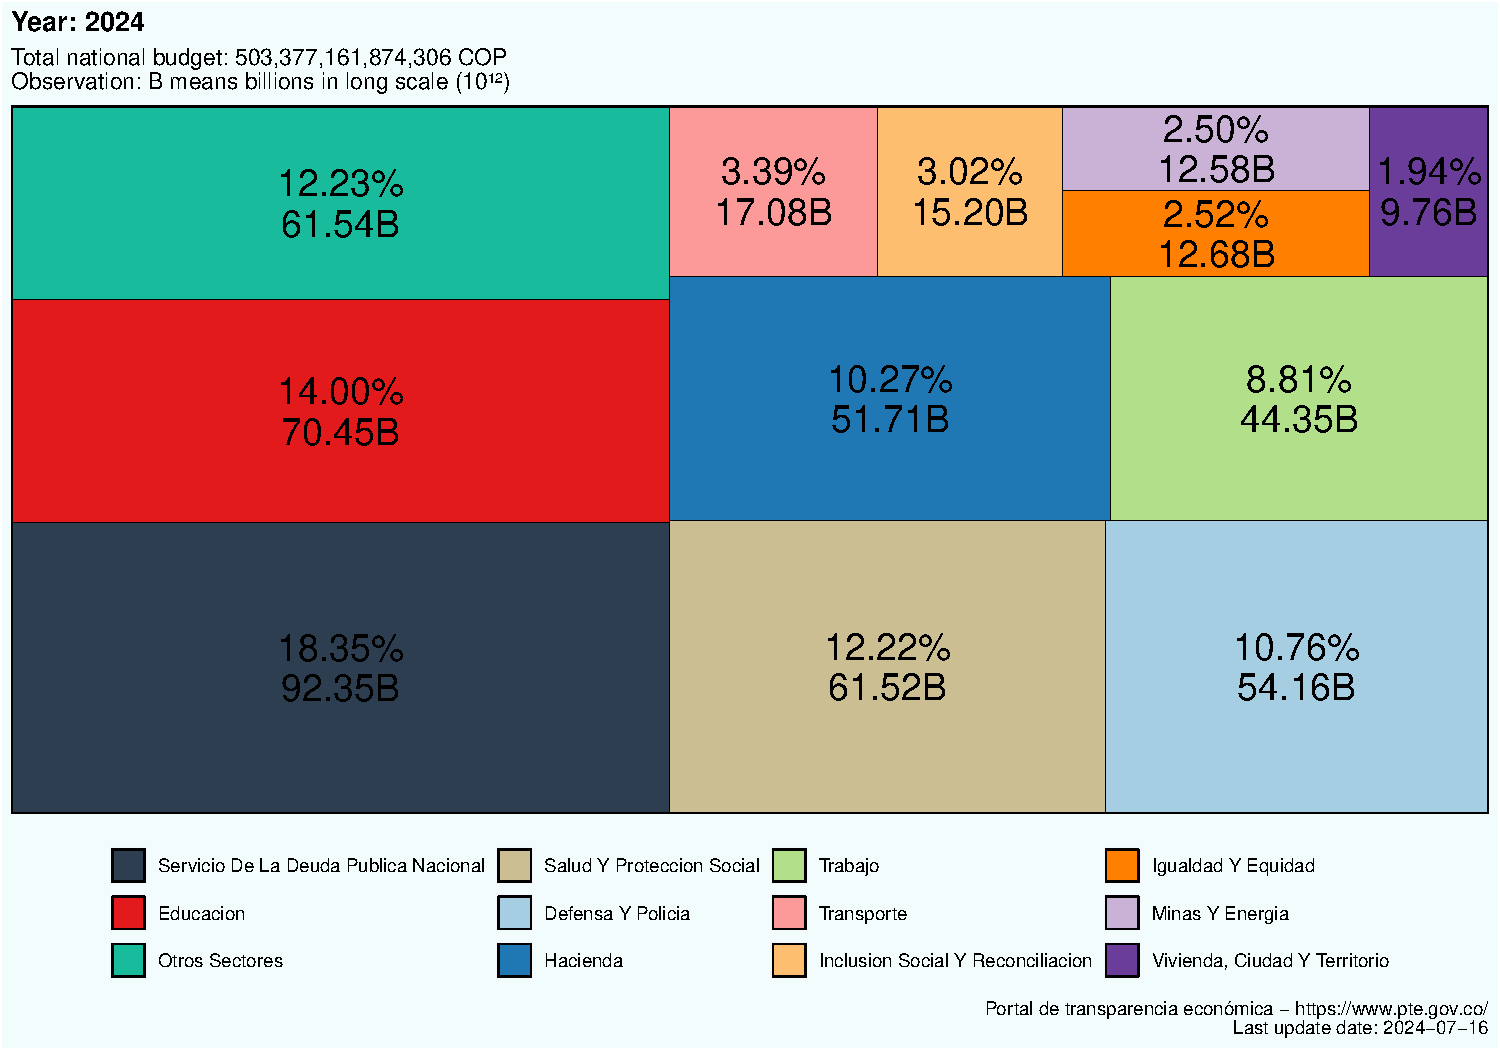
\includegraphics[width=0.85\textwidth,height=\textheight]{006_public_finances_files/figure-beamer/fig-pgn-col-1.pdf}

}

\caption{\label{fig-pgn-col}Who spends nation's general budget spent
on?}

\end{figure}%
\end{frame}

\section{Acknowledgments}\label{acknowledgments}

\begin{frame}{}
\phantomsection\label{section-23}
\begin{itemize}
\item
  To my family that supports me
\item
  To the taxpayers of Colombia and the
  \href{https://www.umng.edu.co/estudiante}{\textbf{UMNG students}} who
  pay my salary
\item
  To the \href{https://www.business-science.io/}{\textbf{Business
  Science}} and \href{https://www.rfordatasci.com/}{\textbf{R4DS Online
  Learning}} communities where I learn
  \href{https://www.r-project.org/about.html}{\textbf{R}} and
  \href{https://www.python.org/about/}{\textbf{\(\pi\)-thon}}
\item
  To the \href{https://www.r-project.org/contributors.html}{\textbf{R
  Core Team}}, the creators of
  \href{https://rstudio.com/products/rstudio/}{\textbf{RStudio IDE}},
  \href{https://quarto.org/}{\textbf{Quarto}} and the authors and
  maintainers of the packages
  \href{https://CRAN.R-project.org/package=tidyverse}{\textbf{tidyverse}},
  \href{https://CRAN.R-project.org/package=readxl}{\textbf{readxl}},
  \href{https://CRAN.R-project.org/package=knitr}{\textbf{knitr}},
  \href{https://CRAN.R-project.org/package=kableExtra}{\textbf{kableExtra}},
  \href{https://CRAN.R-project.org/package=tidyquant}{\textbf{tidyquant}},
  \href{https://CRAN.R-project.org/package=janitor}{\textbf{janitor}},
  \href{https://CRAN.R-project.org/package=treemapify}{\textbf{treemapify}},
  and
  \href{https://CRAN.R-project.org/package=tinytex}{\textbf{tinytex}}
  for allowing me to access these tools without paying for a license
\item
  To the \href{https://www.kernel.org/category/about.html}{\textbf{Linux
  kernel community}} for allowing me the possibility to use some
  \href{https://static.lwn.net/Distributions/}{\textbf{Linux
  distributions}} as my main
  \href{https://en.wikipedia.org/wiki/Operating_system}{\textbf{OS}}
  without paying for a license
\end{itemize}
\end{frame}

\section*{References}\label{references}
\addcontentsline{toc}{section}{References}

\begin{frame}[allowframebreaks]{References}
\phantomsection\label{refs}
\begin{CSLReferences}{1}{0}
\bibitem[\citeproctext]{ref-cardenas_introduccion_2020}
Cardenas, Mauricio. 2020. \emph{Introducción a La {Economía}
{Colombiana}}. 4th ed. Alfaomega.

\bibitem[\citeproctext]{ref-ciefp_clasificacion_2021}
CIEFP. 2021. {``Clasificación de Entidades Del {Sector} {Público}
Colombiano Para La Elaboración de {Estadísticas} de {Finanzas}
{Públicas}.''}
\url{https://www.minhacienda.gov.co/webcenter/ShowProperty?nodeId=/ConexionContent/WCC_CLUSTER-159963}.

\bibitem[\citeproctext]{ref-council_for_economic_education_focus_2010}
Education, Council For Economic. 2010. \emph{Focus: {Understanding}
Economics in Civics and Government}. New York, NY.

\bibitem[\citeproctext]{ref-international_monetary_fund_government_2014}
Fund, International Monetary, ed. 2014. \emph{Government Finance
Statistics Manual 2014}. Washington, DC: IMF.

\bibitem[\citeproctext]{ref-oecd_revenue_2020}
OECD. 2020. \emph{Revenue {Statistics} 2020}. Revenue {Statistics}.
OECD. \url{https://doi.org/10.1787/8625f8e5-en}.

\bibitem[\citeproctext]{ref-oecd_government_2021}
---------. 2021. \emph{Government at a {Glance} 2021}. Government at a
{Glance}. OECD. \url{https://doi.org/10.1787/1c258f55-en}.

\bibitem[\citeproctext]{ref-observatorio_fiscal_de_la_universidad_javeriana_guiciudadana_2018}
Universidad Javeriana, Observatorio Fiscal de la. 2018. {``Guía
Ciudadana a La Tributación y El Gasto Del {Estado} Colombiano.''}
\url{https://www.ofiscal.org/publicaciones}.

\bibitem[\citeproctext]{ref-observatorio_fiscal_de_la_universidad_javeriana_guiciudadana_2022}
---------. 2022. {``Guía Ciudadana Al {Presupuesto} {General} de La
{Nación}.''} \url{https://www.ofiscal.org/guiasciudadanas}.

\end{CSLReferences}
\end{frame}




\end{document}
